\documentclass[runningheads,a4paper]{llncs}

\usepackage[utf8]{inputenc}
\usepackage{amssymb}
\setcounter{tocdepth}{3}
\usepackage{graphicx}

\usepackage{url}
\newcommand{\keywords}[1]{\par\addvspace\baselineskip
\noindent\keywordname\enspace\ignorespaces#1}

\renewcommand*\abstractname{Resumo}

\begin{document}

\mainmatter 

\title{Produção e Custos de Armazenamento}
\author{Kevin Amorim e Luís Magalhães}
\institute{FEUP-PLOG\\ Turma XMIEIC Grupo Xpto1}
\maketitle


\begin{abstract}

Trabalho realizado para a cadeira de Programação em Lógica. Para o realizar recorre-se à linguagem de programação Prolog, de forma a podermos aplicar o paradigma da programação em lógica. Recorre-se essencialmente à programaçáo em lógica com restrições com optimização dos resultados encontrados. Com os resultados obtidos viu-se que quanto mais determinadas sáo as restrições aplicadas mais rápida e precisa é a solução retornada. E ainda que, a falta de certas restrições pode levar a não se conseguir obter uma solução em tempo útil.

\keywords{ Prolog, Programação em Lógica, Optimização, Restrições, Custo, Minimização}
\end{abstract}


\section{Introdução}

O trabalho para a cadeira de Programação em Lógica consiste em encontrar uma solução para problemas de produção e custos de armazenamentos em fábricas, e ainda optimizar as soluções. Para a resolução do problema recorre-se ao paradigma da linguagem de programação Prolog, aplicado às restrições. Com este projeto pretende-se perceber a eficácia de Prolog na resolução de problemas de otimização, tanto na facilidade da escrita de uma solução como na sua velocidade de resolução. Existem várias restrições parametrizáveis para o problema, que poderão ser alteradas para a obtenção de diferentes resultados. Além da obtenção de resultados para a resolução do problema faz-se também a otimização desses mesmos resultados, retornando aqueles que garantem um maior lucro para a empresa. 

Este artigo irá descrever mais detalhadamente o problema em questão, assim como a abordagem tomada para a resolução do mesmo. Além disso, apresentará os resultados obtidos e as respetivas conclusões. 

\section{Descrição do Problema}

O problema proposto foca-se em encontrar um plano produção para as fábricas da empresa de forma a satisfazer as necessidades de produção e minimizando os custos de armazenamento. É ainda um requisito obrigatório que se respeite as restrições impostas para cada fábrica e produto. Espera-se ainda que as variáveis do problema sejam parametrizáveis. Isto é, possibilitar a resolução para vários produtos e várias fábricas, com diferentes restrições. 
As fábricas têm uma limitação de produção diária e o custo de produção de cada produto para cada fábrica poderá variar. Além disso, existe um limite de horas de trabalho por fábrica e cada produto tem um custo em horas de trabalho. Poderão existir ainda restrições relativas à proporção de produção de cada produto, dentro de cada fábrica, podendo mesmo algumas fábricas não poderem produzir certos produtos. Para finalizar, a produção dos produtos deverá garantir as vendas diárias expectadas e ainda poder manter um número de produtos em armazenamento, número esse que também é um parâmetro escolhido. 

Tendo em conta todos estes fatores, a solução apresentada deverá respeitar todas as restrições e ainda minimizar os custos de armazenamento e os custos de produção, de forma a aumentar o lucro. 

\section{Abordagem}

\subsection{Variáveis de Decisão}
As variáveis de decisão utilizadas foram: ProductionPerFactoryX, ProductionCostFactoryX [0, MAX], ProductionPerProductX, StorageX [0, MAX], WorkHoursPerFactoryX [0, Horas diárias disponiveis] , em que X = { 1, 2, 3 } e corresponde ao período temporal. 

\subsection{Restrições}
Existem quatro principais categorias de restrições no problema: restrições na produção, no armazenamento, nas horas de trabalho e no custo. Para as restrições de produção verificámos quais os produtos que cada fábrica não pode produzir em determinado período, restrição esta que é parametrizável. Para a mesma categoria tem-se em conta as restrições da proporção de produção de cada produto em relação aos outros, para cada fábrica, esta também flexível. 

As restrições de armazenamento garantem que no final de cada período haja um determinado número de exemplares de cada produto em stock, número este que é parametrizável. 

As restrições de horas de trabalho pretendem garantir que o número de horas gasto na produção dos produtos não ultrapasse o número de horas disponíveis para cada fábrica. O custo em horas de trabalho de cada produto, assim como as horas disponíveis para cada fábrica podem ser alteradas, o que torna a restrição flexível. 

Por fim, o custo monetário de produção de cada produto também é parametrizável. Esta restrição é importante para a posterior otimização do custo de produção dos produtos, pela empresa, de modo a aumentar o seu lucro. 

\subsection{Função de Avaliação}

A solução obtida pelo predicado solve, atendendo a todas as restrições e parámetros iniciais é posteriormente avaliada tentando minimizar a variável Cost.  No predicado `solve' que trata da obtenção de uma solução para o problema é primeiramente avaliadas todas as restrições. Obtido a produção por período é calculado o custo monetário que essa mesma produção irá ter para cada período, sendo de seguida somado o custo de todos os período por forma a obter um custo total para aquele ano, valor guardado na variável `Cost'. No labeling é feito o minimize dessa mesma variável, com o objetivo de minimizar o custo de produção e aumentar o lucro para a empresa. 

\subsection{Estratégia de Pesquisa}

Foi utilizado a estratégia de etiquetagem por defeito, sendo apenas aplicado a minimização e um timeout à mesma.


\section{Visualização da Solução}

Para a apresentação dos resultados em modo de texto utiliza-se o predicado `print2'. Este predicado imprime na consola a informação relativa a um determinado período. Para o efeito recebe como parâmetros o período correspondente, a produção por fábrica, o custo da produção por fábrica, o armazenamento inicial, a produção por produto, as vendas por produto, o armazenamento final e o número total de horas de trabalho por fábrica. Toda esta informação é imprimida na consola de forma legível e compreensível, com cada valor devidamente identificado. 

\section{Resultados}

Criou-se três casos de teste, com complexidades diferentes para demonstrar a variação dos resultados obtidos com o tempo de resolução. 

Para o primeiro caso utilizou-se cinco fábricas e três produtos com 120 horas diárias de trabalho disponíveis. Para este caso começamos com um timeout de 1 minuto, que nos retorna um custo de produção de 10319 u.m.. Aumentando o timeout para resolução para 60 minutos conseguimos reduzir o custo de produção para 10309 u.m.. Conclui-se então que ao fim de 1 minutos encontramos uma solução praticamente otimizada, para este caso. 

Para o segundo caso temos 3 fábricas e 2 produtos, com 100 horas diárias de trabalho disponíveis. Neste caso, começamos com um timeout de 1 minuto, em que obtemos um custo de 2160 u.m.. Aumentando gradualmente o timeout até 10 minutos o custo de produção retornado manteve-se sempre no mesmo valor, pelo que concluímos que conseguimos obter uma solução completamente otimizada logo à partida.

Para o último caso temos 2 fábricas e 4 produtos, com 100 horas diárias de trabalho disponíveis. Começamos igualmente com um timeout de 1 minuto, obtendo um custo de produção de 9484 u.m.. Aumentamos depois o timeout para 2 minutos vindo a obter um custo de produção de 9416 u.m.. Por fim, com um timeout de 10 minutos, obtemos um custo de produção de 9280 u.m., podendo concluir que neste caso o aumento do timeout trouxe uma otimização considerável no custo de produção. 


Apresentam-se 3 gráficos comparativos dos resultados obtidos nas 3 experiências: 

\begin{figure}[ht!]
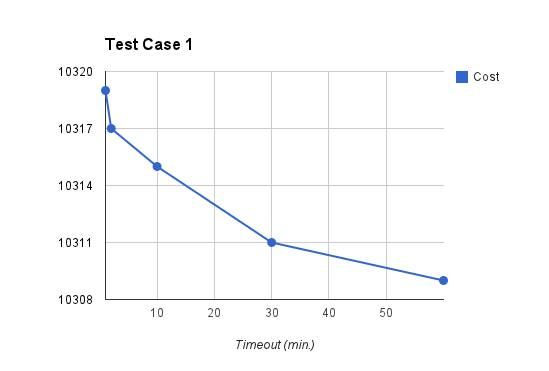
\includegraphics[width=90mm]{test1.jpg}
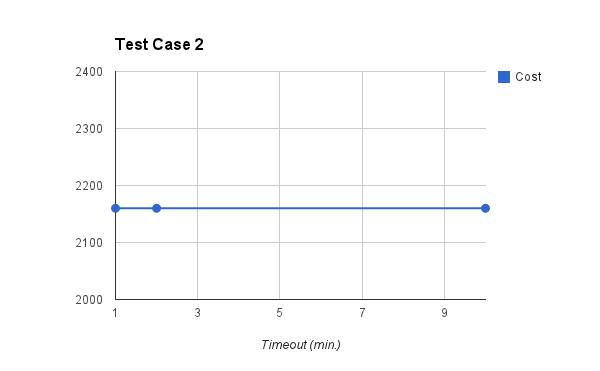
\includegraphics[width=90mm]{test2.jpg}
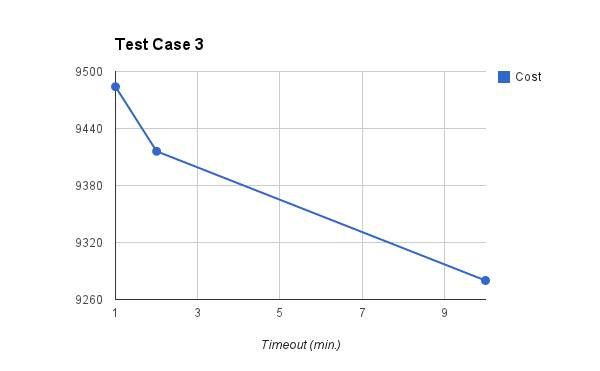
\includegraphics[width=90mm]{test3.jpg}
\end{figure}





\section{Conclusões}





\section{The References Section}\label{references}

In order to permit cross referencing within LNCS-Online, and eventually
between different publishers and their online databases, LNCS will,
from now on, be standardizing the format of the references. This new
feature will increase the visibility of publications and facilitate
academic research considerably. Please base your references on the
examples below. References that don't adhere to this style will be
reformatted by Springer. You should therefore check your references
thoroughly when you receive the final pdf of your paper.
The reference section must be complete. You may not omit references.
Instructions as to where to find a fuller version of the references are
not permissible.

We only accept references written using the latin alphabet. If the title
of the book you are referring to is in Russian or Chinese, then please write
(in Russian) or (in Chinese) at the end of the transcript or translation
of the title.

The following section shows a sample reference list with entries for
journal articles \cite{jour}, an LNCS chapter \cite{lncschap}, a book
\cite{book}, proceedings without editors \cite{proceeding1} and
\cite{proceeding2}, as well as a URL \cite{url}.
Please note that proceedings published in LNCS are not cited with their
full titles, but with their acronyms!

\begin{thebibliography}{4}

\bibitem{jour} Smith, T.F., Waterman, M.S.: Identification of Common Molecular
Subsequences. J. Mol. Biol. 147, 195--197 (1981)

\bibitem{lncschap} May, P., Ehrlich, H.C., Steinke, T.: ZIB Structure Prediction Pipeline:
Composing a Complex Biological Workflow through Web Services. In: Nagel,
W.E., Walter, W.V., Lehner, W. (eds.) Euro-Par 2006. LNCS, vol. 4128,
pp. 1148--1158. Springer, Heidelberg (2006)

\bibitem{book} Foster, I., Kesselman, C.: The Grid: Blueprint for a New Computing
Infrastructure. Morgan Kaufmann, San Francisco (1999)

\bibitem{proceeding1} Czajkowski, K., Fitzgerald, S., Foster, I., Kesselman, C.: Grid
Information Services for Distributed Resource Sharing. In: 10th IEEE
International Symposium on High Performance Distributed Computing, pp.
181--184. IEEE Press, New York (2001)

\bibitem{proceeding2} Foster, I., Kesselman, C., Nick, J., Tuecke, S.: The Physiology of the
Grid: an Open Grid Services Architecture for Distributed Systems
Integration. Technical report, Global Grid Forum (2002)

\bibitem{url} National Center for Biotechnology Information, \url{http://www.ncbi.nlm.nih.gov}

\end{thebibliography}


\section*{Appendix: Springer-Author Discount}

LNCS authors are entitled to a 33.3\% discount off all Springer
publications. Before placing an order, the author should send an email, 
giving full details of his or her Springer publication,
to \url{orders-HD-individuals@springer.com} to obtain a so-called token. This token is a
number, which must be entered when placing an order via the Internet, in
order to obtain the discount.

\section{Checklist of Items to be Sent to Volume Editors}
Here is a checklist of everything the volume editor requires from you:


\begin{itemize}

\item The final \LaTeX{} source files
\item A final PDF file
\item A copyright form, signed by one author on behalf of all of the
authors of the paper.
\item A readme giving the name and email address of the
corresponding author.
\end{itemize}
\end{document}
